\documentclass[onlytextwidth, aspectratio=169]{beamer}
\usepackage[utf8]{inputenc}
\usepackage{microtype}
\usepackage{amsmath}
\usepackage{amssymb}
\usepackage[nomessages]{fp} %\FPeval{\var-name}{2*sin(pi/6)}
\usepackage{siunitx} %units in math. eg 20\milli\meter
\usepackage{yhmath} % for arcs, overparenth command
\usepackage{tikz} %graphics
\usetikzlibrary{quotes, angles, arrows, arrows.meta}
%\usepackage{graphicx} already loaded by beamer class
%consider setting \graphicspath{{images/}}
%\parskip ?? to avoid paragraph indent
\usepackage{multicol} %may not need this package, just columns environment
\usepackage{venndiagram}

\subtitle[BECA]{Bronx Early College Academy}
\author[Huson]{Christopher J. Huson PhD}

\setbeamertemplate{headline}{\vskip2mm 
  \, BECA / \insertshortauthor \, / \inserttitle
  \hfill 
  \insertsection
  }

%Tick mark commands
\newcommand\ticks{}
  \def\ticks{{Bar[scale=2]}-{Bar[scale=2]}}
\newcommand\paraticks{}
  \def\paraticks{{Straight Barb[reversed, scale=2]}-{Straight Barb[scale=2]}}

\title{Geometry Unit 3: Transversals}
\date{11 October - 21 October 2022}

\begin{document}
\frame{\titlepage}
\section[Outline]{}
\frame{\tableofcontents}

\section{3.1 Identify transversal angles \hfill 17 October \,}
\begin{frame}{Learning Target: I can name parallel lines transversal angles}
  {HSG.CO.C.9 Prove theorems about lines and angles  \hfill \alert{3.1 Monday 17 October}}
  \begin{block}{Do Now: Identify the true statements}
    \begin{multicols}{2}
    \begin{enumerate}
      \item $\angle 1 \cong \angle 2$
      \item $\angle 2 \cong \angle 4$
      \item m$\angle 1 + \text{m}\angle 4=180^\circ$
      \item m$\angle 2 + \text{m}\angle 3=90^\circ$
    \end{enumerate}
    \begin{center}
    \begin{tikzpicture}[scale=1, rotate=0]
      \draw[<->, thick] (0:-2)--(0:2);
      \draw[<->, thick] (70:-2)--(70:2);
      \node at (120:0.8){1};
      \node at (35:1.2){2};
      \node at (-55:1){3};
      \node at (35:-1.2){4};
    \end{tikzpicture}
    \end{center}
  \end{multicols}
  \end{block}
    Lesson: Parallel lines crossed by a transverse line, horizontal and vertical directions
\end{frame}

\begin{frame}{New terminology for parallel lines}
  {Parallel lines are in the same plane and never intersect}
    \begin{columns}
      \column{0.6\textwidth}
      \begin{description}
        \item[Parallel lines] $j \parallel k$, mark with arrows
        \item[Transversal] Line  $l$, crosses parallel lines
        \item[Interior] Inside ($\angle$s)
        \item[Exterior] Outside ($\angle$s)
        \item[Same side] On the left or right of $l$
        \item[Alternate] Across $l$ from each other
        \item[Horizontal] Sideways direction
        \item[Vertical] Up and down direction
      \end{description}
      \column{0.4\textwidth}
        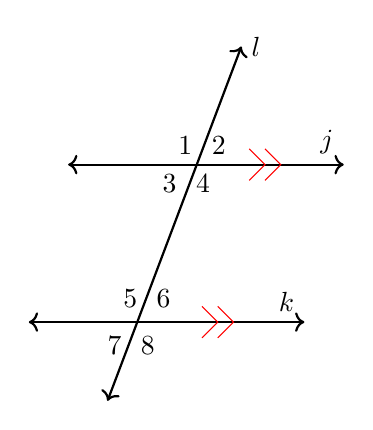
\begin{tikzpicture}[scale=1]
        \draw[<->, thick] (3.5,2)--(7,2)node[above left]{$j$};
        \draw[<->, thick] (3,0)--(6.5,0)node[above left]{$k$};
        \draw[<->, thick] (4,-1)--(5.7,3.5)node[right]{$l$};
        \draw[red] (5.2,-0.2)--(5.4,0)--(5.2,0.2);
        \draw[red] (5.4,-0.2)--(5.6,0)--(5.4,0.2);
        \draw[red] (5.8,1.8)--(6,2)--(5.8,2.2);
        \draw[red] (6,1.8)--(6.2,2)--(6,2.2);
      \onslide<2->
        \node at (4.5,0.3) [left]{$5$};
        \node at (4.5,0.3) [right]{$6$};
        \node at (4.3,-0.3) [left]{$7$};
        \node at (4.3,-0.3) [right]{$8$};
        \node at (5.2,2) [above left]{$1$};
        \node at (5.2,2) [above right]{$2$};
        \node at (5,2) [below left]{$3$};
        \node at (5,2) [below right]{$4$};
      \end{tikzpicture}
    \end{columns} \vspace{0.5cm}
    \onslide<2->
    {\flushright{We often number the angles this way.}}
  \end{frame}

\begin{frame}{New theorems for parallel lines}
  \begin{description}
    \item[Corresponding]  Having the same position. e.g. $\angle 2$ and $\angle 6$
    \item[Postulate] Corresponding $\angle$s of $\parallel$ lines are congruent, 
    $\angle 2 \cong \angle 6$
  \end{description} \bigskip
    \begin{columns}
    \column{0.6\textwidth}
      \begin{enumerate}
        \item Alternate interior  $\angle$s are $\cong$\\
        $\angle 4 \cong \angle 5$
        \item Same-side interior $\angle$s are supplementary\\
        m$\angle 3 + \text{m}\angle 5 =  180$
        \item Alternate exterior  $\angle$s are $\cong$\\
        $\angle 1 \cong \angle 8$
      \end{enumerate}
    \column{0.4\textwidth}
      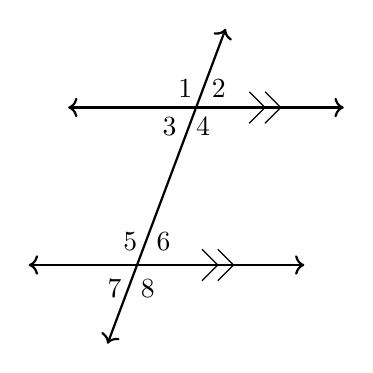
\begin{tikzpicture}[scale=1]
      \draw[<->, thick] (3.5,2)--(7,2);
      \draw[<->, thick] (3,0)--(6.5,0);
      \draw[<->, thick] (4,-1)--(5.5,3);
      \draw (5.2,-0.2)--(5.4,0)--(5.2,0.2);
      \draw (5.4,-0.2)--(5.6,0)--(5.4,0.2);
      \draw (5.8,1.8)--(6,2)--(5.8,2.2);
      \draw (6,1.8)--(6.2,2)--(6,2.2);
      \node at (4.5,0.3) [left]{$5$};
      \node at (4.5,0.3) [right]{$6$};
      \node at (4.3,-0.3) [left]{$7$};
      \node at (4.3,-0.3) [right]{$8$};
      \node at (5.2,2) [above left]{$1$};
      \node at (5.2,2) [above right]{$2$};
      \node at (5,2) [below left]{$3$};
      \node at (5,2) [below right]{$4$};
      \end{tikzpicture}
    \end{columns} \vspace{0.7cm}
    There are only two angle measures, the acute $\angle$s and the obtuse $\angle$s \\
    And they add to $180^\circ$, i.e. supplementary
  \end{frame}

\begin{frame}{Apply the theorems of parallel lines with a transversal}
  Given two parallel lines and a transversal, with m$\angle 6 =  70^\circ$. Write down the value of each angle measure.
  \begin{multicols}{2}
    \begin{enumerate}
      \item m$\angle 1 = $
      \item m$\angle 2 = $
      \item m$\angle 3 = $
      \item m$\angle 4 = $
      \item m$\angle 5 = $
      \item m$\angle 6 = 70^\circ$
      \item m$\angle 7 = $
      \item m$\angle 8 = $
    \end{enumerate}
      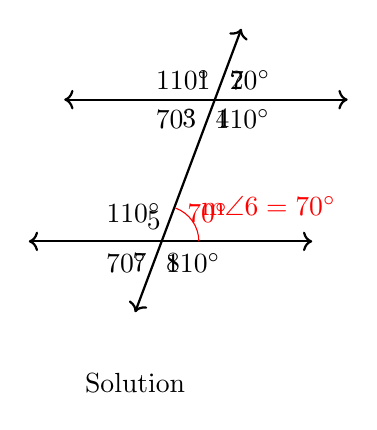
\begin{tikzpicture}[scale=0.9]
      \draw[<->, thick] (3,2)--(7,2);
      \draw[<->, thick] (2.5,0)--(6.5,0);
      \draw[<->, thick] (4,-1)--(5.5,3);
      \onslide<1>
      {\node at (4.8,0.5) [red, right]{m$\angle 6 = 70^\circ$};
      \draw[red] (4.9,0) arc (0:70:0.5);
      \node at (4.5,0.3) [left]{$5$};
      \node at (4.3,-0.3) [left]{$7$};
      \node at (4.3,-0.3) [right]{$8$};
      \node at (5.2,2) [above left]{$1$};
      \node at (5.2,2) [above right]{$2$};
      \node at (5,2) [below left]{$3$};
      \node at (5,2) [below right]{$4$};}
      \onslide<2>
      {\node at (4.6,0.4) [red, right]{$70^\circ$};
      \node at (4.5,0.4) [left]{$110^\circ$};
      \node at (4.3,-0.3) [left]{$70^\circ$};
      \node at (4.3,-0.3) [right]{$110^\circ$};
      \node at (5.2,2) [above left]{$110^\circ$};
      \node at (5.2,2) [above right]{$70^\circ$};
      \node at (5,2) [below left]{$70^\circ$};
      \node at (5,2) [below right]{$110^\circ$};
      \node at (4,-2){Solution};}
    \end{tikzpicture}
  \end{multicols}
\end{frame}

\begin{frame}{Extension: Ratios are fractions}
  {We often state proportions as ratios}
  Example: Divide a distance into equal parts, i.e. $$1:1$$ 
  We say ``one to one'', or ``in a one to one ratio.''\\
A rectangle's length to width ratio is two to one. $2:1$
\end{frame}

\section{3.2 Transversals problems \hfill 18 October \,}
\begin{frame}{Learning Target: I can calculate transversal angles}
  {HSG.CO.C.9 Prove theorems about lines and angles  \hfill \alert{3.2 Tuesday 18 October}}
  \begin{block}{Do Now: Identify each angle}
    \begin{multicols}{2}
    \begin{enumerate}
      \item Opposite $\angle 4$
      \item Corresponding to $\angle 3$
      \item Alternate exterior to $\angle 8$
      \item Same side interior to $\angle 5$
      \item Alternate interior to $\angle 4$
  \end{enumerate}
  \begin{center}
    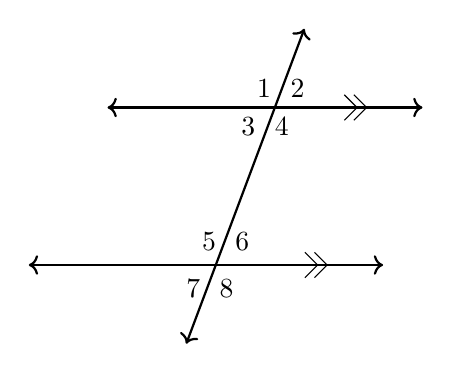
\begin{tikzpicture}[scale=1]
      \draw[<->, thick] (3,2)--(7,2);
      \draw[<->, thick] (2,0)--(6.5,0);
        \draw[\paraticks] (6,2)--(6.3,2);
        \draw[\paraticks] (5.5,0)--(5.8,0);
      \draw[<->, thick] (4,-1)--(5.5,3);
      \node at (4.5,0.3) [left]{$5$};
      \node at (4.5,0.3) [right]{$6$};
      \node at (4.3,-0.3) [left]{$7$};
      \node at (4.3,-0.3) [right]{$8$};
      \node at (5.2,2) [above left]{$1$};
      \node at (5.2,2) [above right]{$2$};
      \node at (5,2) [below left]{$3$};
      \node at (5,2) [below right]{$4$};
    \end{tikzpicture}
  \end{center}
\end{multicols}
\end{block}
Lesson: Solve for angle measures
\end{frame}

%Template
\begin{frame}{Parallel lines intersected by a transversal. Find $x$.}
  Alternate interior angles measure $100^\circ$ and $12x+16$, as shown.
  \begin{flushleft}
    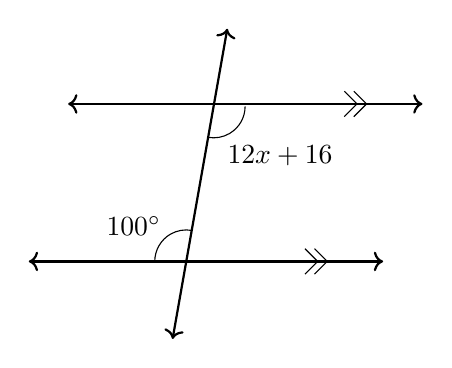
\begin{tikzpicture}[scale=1]
      \draw[<->, thick] (-1.5,2)--(3,2);
      \draw[<->, thick] (-2,0)--(2.5,0);
        \draw[\paraticks] (2,2)--(2.3,2);
        \draw[\paraticks] (1.5,0)--(1.8,0);
      \draw[<->, thick] (80:-1)--(80:3);
      \draw (-0.4,0) arc (180:80:0.4);
      \draw (0.4,0)++(80:2) arc (0:-100:0.4);
      \node at (0,0)[above left=2mm]{$100^\circ$};
      \node at (0,0)[yshift=2cm, below right=4mm]{$12x+16$};
    \end{tikzpicture}
    \end{flushleft} \vspace{1cm}
    Are the angles congruent or supplementary?
\end{frame}

\begin{frame}{Parallel lines intersected by a transversal. Find $x$.}
  {Parallel lines do not have to be horizontal.}
  \begin{flushleft}
    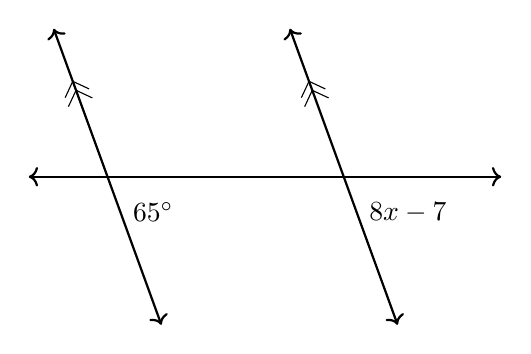
\begin{tikzpicture}[scale=1]
      \draw[<->, thick] (-1,0)--(5,0);
      \draw[<->, thick] (110:-2)--(110:2);
      \draw[<->, thick, xshift=3cm] (110:-2)--(110:2);
        \draw[\paraticks] (110:1)--+(110:0.3);
        \draw[\paraticks, xshift=3cm] (110:1)--+(110:0.3);
      \node at (0,0)[below right=0.2cm]{$65^\circ$};
      \node at (0,0)[xshift=3cm, below right=0.2cm]{$8x-7$};
    \end{tikzpicture}
    \end{flushleft}
    State the postulate or theorem you are employing.
\end{frame}

%Template
\begin{frame}{Parallel lines intersected by a transversal. Find $x$.}
  Given: Same side interior angles measure $115^\circ$ and $15x-10$.
  \begin{flushleft}
    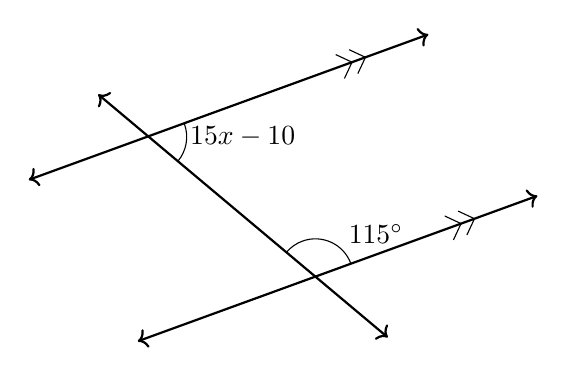
\begin{tikzpicture}[scale=1.2, rotate=20]
      \draw[<->, thick] (-2.5,2)--(2,2);
      \draw[<->, thick] (-2,0)--(2.5,0);
        \draw[\paraticks] (1,2)--(1.3,2);
        \draw[\paraticks] (1.5,0)--(1.8,0);
      \draw[<->, thick] (1200:-1)--(120:3);
      \draw (0.4,0) arc (0:120:0.4);
      \draw (0.4,0)++(120:2.3) arc (0:-60:0.4);
      \node at (0,0)[above right=3mm]{$115^\circ$};
      \node at (120:2.3)[right=4mm]{$15x-10$};
    \end{tikzpicture}
    \end{flushleft} \vspace{1cm}
    Remember the check.
\end{frame}

\begin{frame}{Extension: \emph{Partitioning} a segment or angle in a ratio}
  Point $B$ divides $\overline{AC}$ in a $2:1$ ratio, i.e. $AB=2 BC$ \\
  Ray $\overrightarrow{BD}$ divides $\angle ABC$ in a $2:1$ ratio. Find $x$.
  
\end{frame}

\section{3.3 Triangle sum theorem \hfill 20 October \,}
\begin{frame}{Learning Target: I can calculate triangle angles}
{HSG.CO.C.9 Prove theorems about lines and angles  \hfill \alert{3.3 Thursday 20 October}}
  Do Now: 
  \begin{columns}
  \column{0.6\textwidth}
    \begin{enumerate}
      \item Given two parallel lines, two transversals
      \item Find $x$, $y$
      \item What relationship are you using? (e.g. vertical angles, same-side exterior angles, alternate interior angles)
    \end{enumerate}
  \column{0.4\textwidth}
    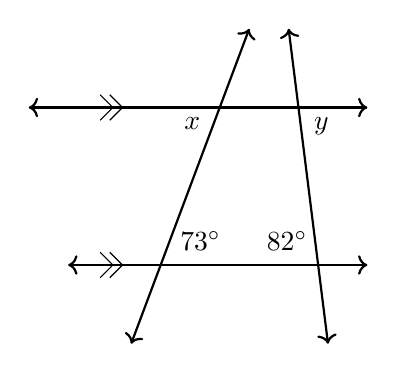
\begin{tikzpicture}[scale=1]
    \draw[<->, thick] (2.7,2)--(7,2);
    \draw[<->, thick] (3.2,0)--(7,0);
      \draw[\paraticks] (3.6,0)--(3.9,0);
      \draw[\paraticks] (3.6,2)--(3.9,2);
    \draw[<->, thick] (4,-1)--(5.5,3);
    \draw[<->, thick] (6.5,-1)--(6,3);
    \node at (4.5,0.3) [right]{$73^\circ$};
    \node at (5.6,0.3) [right]{$82^\circ$};
    \node at (5,2) [below left]{$x$};
    \node at (6.2,2) [below right]{$y$};
    \end{tikzpicture}
  \end{columns} \vspace{0.8cm}
  Lesson: The sum of a triangle's \emph{interior} angles is $180^\circ$ \par \medskip 
  \hspace{1.2cm} \emph{Triangle sum theorem}
\end{frame}

\begin{frame}{Triangle sum theorem}
  Given parallel lines $k \parallel l$, $\triangle ABC$, m$\angle B=65^\circ$, m$\angle C=55^\circ$. \par \smallskip
  Find m$\angle BAC = x$.
  \begin{flushright}
  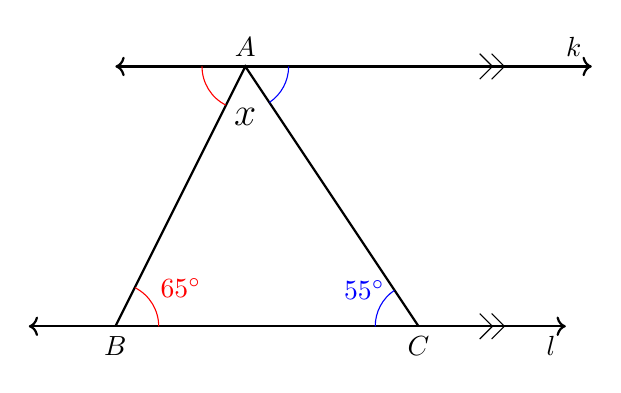
\begin{tikzpicture}[scale=1.1]
    \draw[<->, thick] (0,3)--(5.5,3)node[above left]{$k$};
    \draw[<->, thick] (-1,0)--(5.2,0)node[below left]{$l$};
      \draw[\paraticks] (4.2,3)--(4.5,3);
      \draw[\paraticks] (4.2,0)--(4.5,0);
    \draw[thick] (0,0) node[below]{$B$}--
      (1.5,3) node[above]{$A$}node[below=4mm]{\Large{$x$}}--
      (3.5,0) node[below]{$C$};
    \draw[red] (0.5,0) arc (0:63:0.5)node[right=2mm]{$65^\circ$};
    \draw[red] (1.0,3) arc (0:63:-0.5);%node[above right]{$70^\circ$};
    \draw[blue] (3,0) arc (0:-56:-0.5)node[left]{$55^\circ$};
    \draw[blue] (2,3) arc (0:-56:0.5);%node[left]{$55^\circ$};
  \end{tikzpicture}
  \end{flushright} \bigskip
  \begin{description}
    \item[Interior] The three angles that are \emph{inside} the triangle
    \item[Theorem] The sum of the measures of the three internal angles of a triangle is $180^\circ$
  \end{description}
  \end{frame}

\begin{frame}{Mark 3 missing angle measures to make a straight angle}
  An \emph{auxilary} line $l$ is drawn through $A$, parallel to triangle base $\overline{BC}$. \par \smallskip
  Find m$\angle BAC$. \bigskip
  \begin{columns}
  \column{0.57\textwidth}
    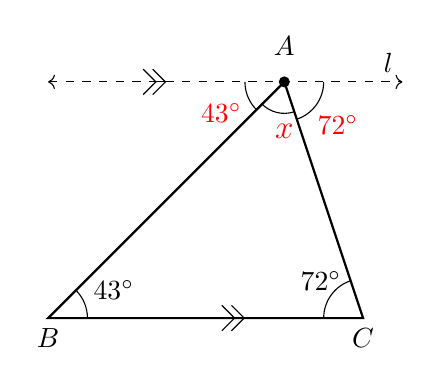
\begin{tikzpicture}[scale=1]
      \draw[<->, dashed] (0,3)--(4.5,3)node[above left]{$l$};
        \draw[\paraticks] (1.2,3)--(1.5,3);
        \draw[\paraticks] (2.2,0)--(2.5,0);
      \draw[thick] (0,0) node[below]{$B$}--
        (3,3) node[above=2mm]{$A$}node[red,below=4mm]{\large{$x$}}--
        (4,0) node[below]{$C$}--cycle;
      \fill (3,3) circle [radius=0.7mm];
      \draw (0.5,0) arc (0:45:0.5)node[right=1mm]{$43^\circ$};
      \draw (2.5,3) arc (0:45:-0.5);
      \draw (3.5,0) arc (0:-72:-0.5)node[left]{$72^\circ$};
      \draw (3.5,3) arc (0:-72:0.5);
      \draw (3,3)++(43:-0.4) arc (223:288:0.4);
      \onslide<2>
        \node at (2.2,2.6)[red]{$43^\circ$};
        \node at (3,3)[red,below right=3mm]{$72^\circ$};
    \end{tikzpicture}
  \column{0.43\textwidth}
    \onslide<2>{
      $43+x+72 = 180$ \par \bigskip
      \hspace{1.7cm} $x = 65^\circ$ \par \bigskip
      Theorem: m$\angle A + \text{m}\angle B + \text{m}\angle C = 180^\circ$ \par
      for any triangle }
  \end{columns} \bigskip
  \begin{description}
    \item[Auxilary] An extra line added to a diagram
    \item[Linear triple] Three adjacent angles that make a straight line
  \end{description}
  \end{frame}

\begin{frame}{Find the missing angle measure}
  Given $\triangle ABC$, m$\angle A=82^\circ$, m$\angle C=59^\circ$. Find  m$\angle B$. \vspace{1cm}
  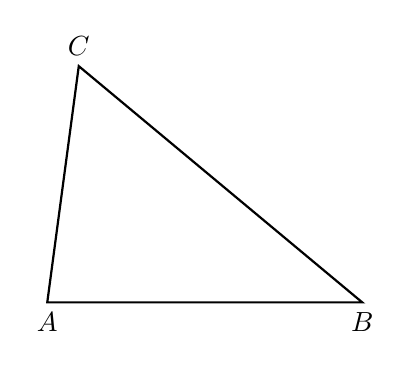
\begin{tikzpicture}
    \draw[thick] (0,0)node[below]{$A$}--
      (4,0)node[below]{$B$}--
      (0.4,3)node[above]{$C$}--cycle;
  \end{tikzpicture}
\end{frame}

\begin{frame}{Triangle sum theorem ($180^\circ$)}
  {Check your notes}
    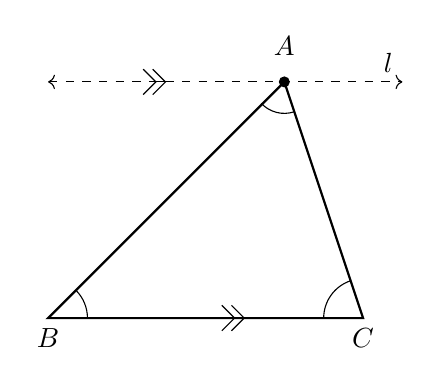
\begin{tikzpicture}[scale=1]
      \draw[<->, dashed] (0,3)--(4.5,3)node[above left]{$l$};
        \draw[\paraticks] (1.2,3)--(1.5,3);
        \draw[\paraticks] (2.2,0)--(2.5,0);
      \draw[thick] (0,0) node[below]{$B$}--
        (3,3) node[above=2mm]{$A$}--
        (4,0) node[below]{$C$}--cycle;
      \fill (3,3) circle [radius=0.7mm];
      \draw (0.5,0) arc (0:45:0.5);
      \draw (3.5,0) arc (0:-72:-0.5);
      \draw (3,3)++(43:-0.4) arc (223:288:0.4);
    \end{tikzpicture} \smallskip
  \begin{description}
    \item[Auxilary line] An extra line added to a diagram
    \item[Linear triple] Three adjacent angles that make a straight line
    \item[Interior angles] The three angles that are inside the triangle
    \item[Theorem] The sum of a triangle's angles is $180^\circ$ \par \smallskip
    m$\angle A + \text{m}\angle B + \text{m}\angle C = 180^\circ$
  \end{description}
  \end{frame}

\begin{frame}{Extension: Euclid's fifth postulate (the \href{https://mathworld.wolfram.com/ParallelPostulate.html}{Parallel Postulate})}
  {Given a line and a point, there exists one line through the point parallel to the line.}
    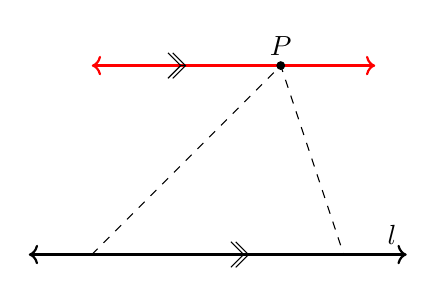
\begin{tikzpicture}[scale=0.8]
      \draw[red,thick,<->] (0,3)--(4.5,3); %node[above left]{$l$};
        \draw[\paraticks] (1.2,3)--(1.5,3);
        \draw[\paraticks] (2.2,0)--(2.5,0);
      \draw[<->,thick] (-1,0)--(5,0) node[above left]{$l$};
      \draw[dashed] (0,0)--(3,3)--(4,0);
      \fill (3,3) circle [radius=0.7mm] node[above]{$P$};
    \end{tikzpicture} \smallskip
  \begin{description}
    \item[Euclid] Greek author of the most successful math book of all time, \emph{The Elements}
    \item[Postulate] A statement we assume is true as the basis of all further mathematical theorems and proofs
    \item[Non-Euclidean geometries] Alternative mathematics not using the Parallel Postulate. Lobachevsky (1826 Russian), Bolyai (1832 Hungarian), Einstein (1916 German)
  \end{description}
  \end{frame}

\section{3.4 Parallelograms \hfill 21 October \,}
\begin{frame}{Learning Target: I can find the angles of a parallelogram}
  {HSG.CO.C.9 Prove theorems about lines and angles  \hfill \alert{3.4 Friday 21 October}}
  Do Now: Two parallel lines intersect a transversal. Given corresponding angles  m$\angle 1 = 4.4x - 63$ and m$\angle 2 = 2.8x+9$. \par \medskip
  Find the measure of $\angle 1$. \bigskip
  \begin{columns}
    \column{0.55\textwidth}
    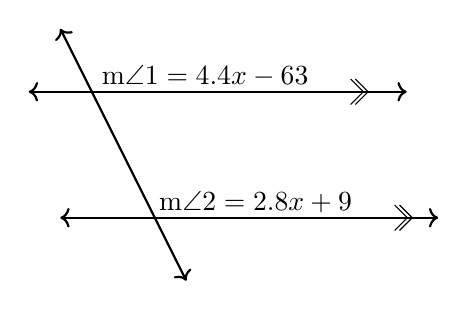
\begin{tikzpicture}[scale=0.8]
      \draw[<->, thick] (3,0)--(9,0);
      \draw[<->, thick] (2.5,2)--(8.5,2);
      \draw[<->, thick] (5,-1)--(3,3);
        \draw[\paraticks] (8.3,0)--(8.6,0);
        \draw[\paraticks] (7.6,2)--(7.9,2);
      \node at (5.3, 2.25){m$\angle 1 = 4.4x - 63$};
      \node at (6.1, 0.25){m$\angle 2 = 2.8x+9$};
    \end{tikzpicture}
    \column{0.45\textwidth}
    \onslide<2> Corresponding angles are $\cong$ \par \medskip
      $4.4x - 63 = 2.8x+9$ \par
      \hspace{0.7cm} $1.6x = 72$ \par
      \hspace{1.2cm} $x = 45$ \par \medskip
      $\text{m}\angle 1 = 4.4(45) - 63=135^\circ$ \par \bigskip
      Check: $\text{m}\angle 2 = 2.8(45)+9=135$
    \end{columns}
\end{frame}

\begin{frame}{A parallelogram's opposite sides are parallel and congruent}
  {Consecutive angles are supplementary. Opposite angles are congruent.}
  Find the other angle measures. \par
    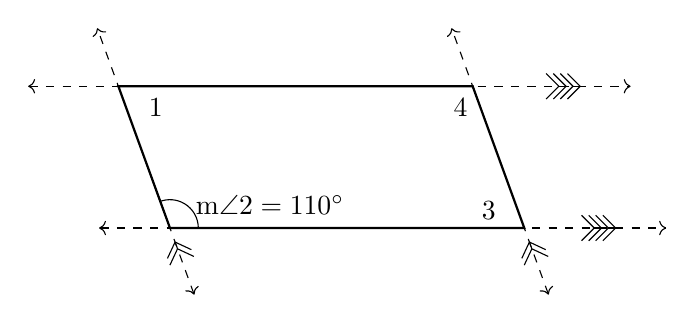
\begin{tikzpicture}[scale=0.9]
      \draw[thick] (0,0)--(110:2.13)--+(5,0)--(5,0)--cycle;
      \draw[<->, dashed] (-1,0)--(7,0);
      \draw[<->, dashed] (-2,2)--(6.5,2);
        \draw[\paraticks] (5.8,0)--+(0.3,0);
        \draw[\paraticks] (6.0,0)--+(0.3,0);
        \draw[\paraticks] (5.3,2)--+(0.3,0);
        \draw[\paraticks] (5.5,2)--+(0.3,0);
      \draw[<->, dashed] (110:-1)--(110:3);
      \draw[<->, dashed, xshift=5cm] (110:-1)--(110:3);
        \draw[\paraticks] (110:-0.5)--+(110:0.3);
        \draw[\paraticks, xshift=5cm] (110:-0.5)--+(110:0.3);
      \node at (-0.2, 1.7){$1$};
      %\node at (1.5, 0.25){m$\angle 2 = 110^\circ$};
      \node at (4.5, 0.25){$3$};
      \node at (4.1, 1.7){$4$};
      \draw (0.4,0) arc (0:110:0.4)node[pos=0.5, right]{m$\angle 2 = 110^\circ$};
    \end{tikzpicture}
\end{frame}

\section{3.5 External angles \hfill 24 October \,}
\begin{frame}{Learning Target: I can calculate external triangle angles}
  {HSG.CO.C.9 Prove theorems about lines and angles  \hfill \alert{3.5 Monday 24 October}}
  Do Now: 
  \begin{columns}
  \column{0.5\textwidth}
    \begin{enumerate}
      \item Given two parallel lines, two transversals
      \item Find $x$, $y$
      \item What relationship are you using? (e.g. vertical angles, same-side exterior angles, alternate interior angles, etc.)
    \end{enumerate}
  \column{0.5\textwidth}
    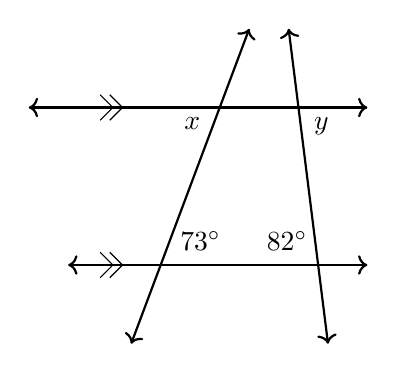
\begin{tikzpicture}[scale=1]
    \draw[<->, thick] (2.7,2)--(7,2);
    \draw[<->, thick] (3.2,0)--(7,0);
      \draw[\paraticks] (3.6,0)--(3.9,0);
      \draw[\paraticks] (3.6,2)--(3.9,2);
    \draw[<->, thick] (4,-1)--(5.5,3);
    \draw[<->, thick] (6.5,-1)--(6,3);
    \node at (4.5,0.3) [right]{$73^\circ$};
    \node at (5.6,0.3) [right]{$82^\circ$};
    \node at (5,2) [below left]{$x$};
    \node at (6.2,2) [below right]{$y$};
    \end{tikzpicture}
  \end{columns}
  Lesson: Triangle external angle theorem
\end{frame}

\begin{frame}
  Given parallel lines $\overleftrightarrow{AB} \parallel \overleftrightarrow{CDE}$ with $\overline{AC} \cong \overline{CD}$. If m$\angle BAD=80$ find m$\angle ACD$.
  \begin{flushright}
  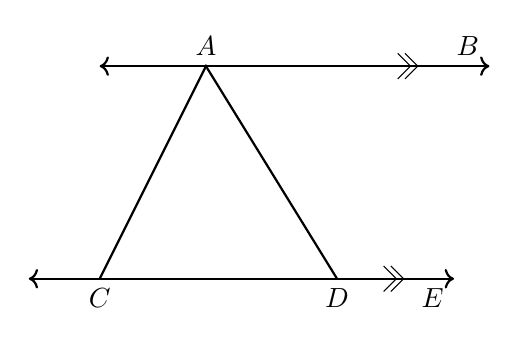
\begin{tikzpicture}[scale=0.9]
    \draw[<->, thick] (1,3)--(6.5,3) node[above left]{$B$};
    \draw[<->, thick] (0,0)--(6,0) node[below left]{$E$};
      \draw[\paraticks] (5.2,3)--(5.5,3);
      \draw[\paraticks] (5,0)--(5.3,0);
    \draw[-, thick] (1,0) node[below]{$C$}--
      (2.5,3) node[above]{$A$}--
      (4.35,0) node[below]{$D$};
  \end{tikzpicture}
  \end{flushright} \vspace{1cm}
  \end{frame}


\section{3.6 Transversal situations \hfill 25 October \,}
\begin{frame}{Learning Target: I can calculate transversal angles (algebra review)}
  {HSG.CO.C.9 Prove theorems about lines and angles  \hfill \alert{3.6 Tuesday 25 October}}
  Given two parallel lines and a transversal, \par \smallskip
    m$\angle 4 = 3x$ and m$\angle 5 = x + 70$. \par \smallskip 
    Write an equation, then solve for $x$.
  \begin{flushright}
    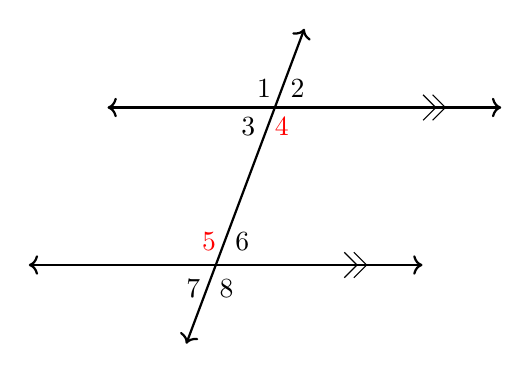
\begin{tikzpicture}[scale=1]
      \draw[<->, thick] (3,2)--(8,2);
      \draw[<->, thick] (2,0)--(7,0);
        \draw[\paraticks] (7,2)--(7.3,2);
        \draw[\paraticks] (6,0)--(6.3,0);
      \draw[<->, thick] (4,-1)--(5.5,3);
      \node at (4.5,0.3) [red, left]{$5$};
      \node at (4.5,0.3) [right]{$6$};
      \node at (4.3,-0.3) [left]{$7$};
      \node at (4.3,-0.3) [right]{$8$};
      \node at (5.2,2) [above left]{$1$};
      \node at (5.2,2) [above right]{$2$};
      \node at (5,2) [below left]{$3$};
      \node at (5,2) [red, below right]{$4$};
    \end{tikzpicture}
  \end{flushright}
\end{frame}

\section{3.7 Parallelogram situations \hfill 27 October \,}
\begin{frame}{Learning Target: I can calculate angles in parallelograms}
  {HSG.CO.C.9 Prove theorems about lines and angles  \hfill \alert{3.7 Wednesday 27 October}}
  Do Now: 
  \begin{multicols}{2}
    \begin{enumerate}
      \item Given a triangle, shown
      \item Find angle measures $x$, $y$
      \item What relationships are you using? (e.g. vertical angles, same-side exterior angles, alternate interior angles)
    \end{enumerate}
    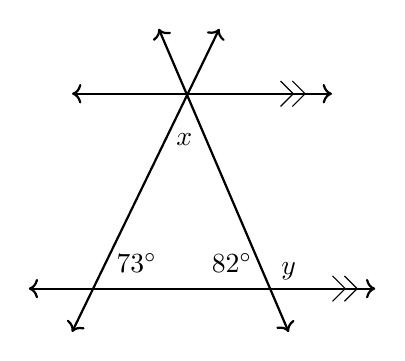
\begin{tikzpicture}[scale=1.1]
      \draw[<->, thick] (4,2.25)--(7,2.25);
      \draw[<->, thick] (3.5,0)--(7.5,0);
        \draw[\paraticks] (6.4,2.25)--(6.7,2.25);
        \draw[\paraticks] (7,0)--(7.3,0);
      \draw[<->, thick] (4,-0.5)--(5.7,3);
      \draw[<->, thick] (6.5,-0.5)--(5,3);
      \node at (4.4,0.3) [right]{$73^\circ$};
      \node at (5.5,0.3) [right]{$82^\circ$};
      \node at (5.5,1.9) [below left]{$x$};
      \node at (6.5,0.2) {$y$};
    \end{tikzpicture}
  \end{multicols}
  Lesson: Triangle's exterior angles
\end{frame}

\section{3.8 Transversals review \hfill 31 October}
\begin{frame}{Learning Target: I can review with my classmates}
  {HSG.CO.C.9 Prove theorems about lines and angles \hfill \alert{3.8 Monday 31 October}}
  Two parallel lines intersect a second set of parallel lines. Given m$\angle 2 = 2.8x+9$ and m$\angle 4 = 4.4x - 63$, find the measure of $\angle 1$. 
  \begin{flushright}
    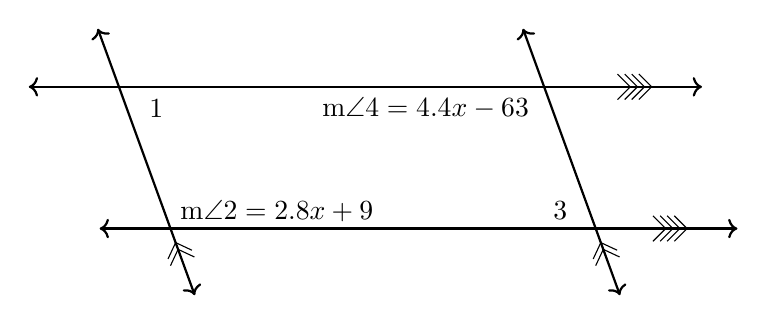
\begin{tikzpicture}[scale=0.9]
      \draw[<->, thick] (-1,0)--(8,0);
      \draw[<->, thick] (-2,2)--(7.5,2);
        \draw[\paraticks] (6.8,0)--+(0.3,0);
        \draw[\paraticks] (7.0,0)--+(0.3,0);
        \draw[\paraticks] (6.3,2)--+(0.3,0);
        \draw[\paraticks] (6.5,2)--+(0.3,0);
      \draw[<->, thick] (110:-1)--(110:3);
      \draw[<->, thick, xshift=6cm] (110:-1)--(110:3);
        \draw[\paraticks] (110:-0.5)--+(110:0.3);
        \draw[\paraticks, xshift=6cm] (110:-0.5)--+(110:0.3);
      \node at (-0.2, 1.7){$1$};
      \node at (1.5, 0.25){m$\angle 2 = 2.8x+9$};
      \node at (5.5, 0.25){$3$};
      \node at (3.6, 1.7){m$\angle 4 = 4.4x - 63$};
    \end{tikzpicture}
    \end{flushright}
\end{frame}

\section{3.9 Transversals test \hfill 1 November}
\begin{frame}{Learning Target: I can review with my classmates}
  {HSG.CO.C.9 Prove theorems about lines and angles \hfill \alert{3.9 Tuesday 1 November \,}}

  \alert{Unit 3 Test: Parallel lines and transversals}

\end{frame}


\end{document}